\section{Proof of Proposition~\ref{prop:closure}}
\label{sec:restriction}

It suffices to prove the proposition for a subsequence of $(H_N)$.
If $\calF'\subseteq\calF$ is the class obtained from a subsequence and
$\equiv_{\calF'}$ coincides with $\equiv_{\mathcal D_3}$, then
$\equiv_{\calF}$ coincides with $\equiv_{\mathcal D_3}$ as well, because
$\calF'\subseteq\calF\subseteq\mathcal D_3$.
Every tail of $(H_N)$ still has unbounded clique-minor size, since a finite
initial segment has bounded clique-minor size. We can therefore choose
and reindex a subsequence so that $H_N$ contains $K_{3N}$ as
a minor for every $N\geq1$; \cref{lem:subdivision-containment} below uses this
property.
We use the subdivision notation $H^{\mathbf m}$ and the labelled
coefficients $c_G(H,\ell)$ from \cref{sec:characterisation}.
For this reindexed sequence, let $\calF'$ consist
of $K_1$ and the graphs $H_N^{\mathbf m}$ for all $N\geq1$ and all tuples $\mathbf m$.

\begin{lemma}\label{lem:subdivision-containment}
 Let $N\geq1$ and suppose that $H_N$ contains $K_{3N}$ as a minor.
 Let $H$ be a connected cubic multigraph with at most $N$ vertices.
 Then $H_N$ contains a subgraph isomorphic to a subdivision of $H$.
\end{lemma}
\begin{proof}
 Since a subdivision of a subdivision of $H$ is a subdivision of $H$, it
 suffices to find a simple subcubic subdivision $J$ of $H$ with at most
 $3N$ vertices. Such a $J$ is a subgraph of $K_{3N}$ and hence a
 minor of $H_N$. Since $J$ is subcubic, it is a topological minor
 of $H_N$~\cite[Section~1.7]{Diestel2017}, so $H_N$ contains a subgraph
 isomorphic to a subdivision of $J$ and hence to a subdivision of $H$.
 Let $J=H^{\mathbf m}$, where $m_e=3$ for each loop, $m_e=2$ for all
 but one edge in each group of parallel non-loop edges, and $m_e=1$
 for all other edges.
 Then $J$ is simple and subcubic. There are two new vertices for each
 loop and $k-1\leq2$ for each group of $k\geq2$ parallel non-loop edges.
 Since $H$ is cubic, these loops and parallel-edge groups have
 disjoint vertex sets. Hence $|V(J)|-|V(H)|\leq2|V(H)|\leq2N$,
 so $J$ has at most $3N$ vertices.
\end{proof}

\begin{lemma}\label{lem:independent-path-lengths}
 Let $H$ be a connected cubic multigraph and let $m\geq1$ be an integer.
 There is a connected cubic graph $D$ with the following property.
 If a graph $X$ contains a subgraph isomorphic to a subdivision of $D$,
 then there are an injection $\iota:V(H)\hookrightarrow V(X)$ and finite
 sets $Q_e\subseteq\Z_{\geq1}$ with $|Q_e|\geq m+1$ for each $e\in E(H)$
 such that, for every $\mathbf q\in\prod_eQ_e$, there is a subdivision
 of $H$ in $X$ with vertex map $\iota$ and paths $R_e$ of lengths $q_e+1$.
 Here $R_e$ is a cycle through $\iota(v)$ if $e$ is a loop at $v$.
 At least one edge of $X$ lies outside the chosen subdivision.
\end{lemma}
\begin{proof}
We construct $D$ by replacing each edge of $H$ by a chain of $m$ diamonds.
The \emph{diamond} $K_4-ab$ is $K_4$ on vertices $a,b,c,d$ with the
edge $ab$ deleted. Its vertices $a,b$ have degree two, and $c,d$ have
degree three. A chain consists of $m$ disjoint copies together with
an edge from $b$ in each copy to $a$ in the next.
For each edge $vw$ of $H$, take a separate chain and add edges from
$v$ to $a$ in its first copy and from $b$ in its last copy to $w$.
The resulting graph $D$ is connected and cubic.
\Cref{fig:diamond-objects} illustrates an example of the construction.
\begin{figure}[tb]
\centering
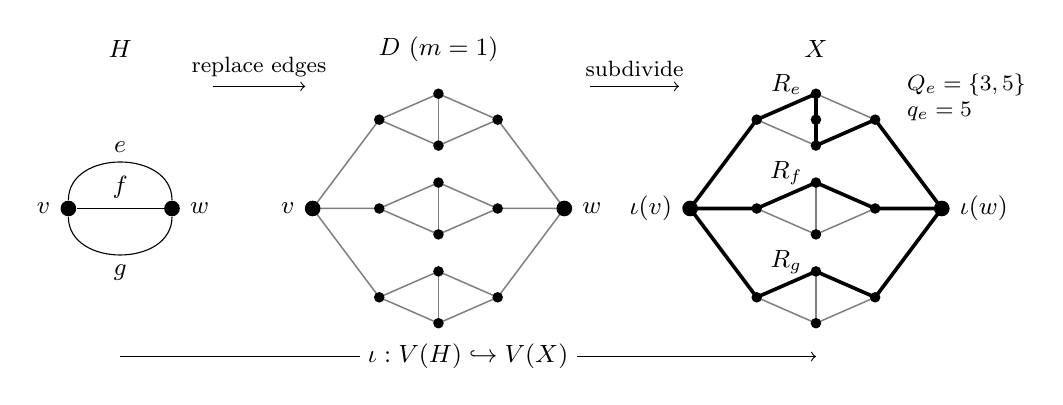
\begin{tikzpicture}[
  x=.94cm,y=.94cm,
  every node/.style={font=\small},
  vertex/.style={circle,fill=black,inner sep=1.35pt},
  branch/.style={circle,fill=black,inner sep=2pt},
  edge/.style={draw=black!50,line width=.55pt},
  chosen/.style={draw=black,line width=1.3pt},
]
\node at (0,2.15) {$H$};
\node at (4.3,2.15) {$D$ ($m=1$)};
\node at (9.4,2.15) {$X$};
\node[branch,label=left:$v$] (hu) at (-.7,0) {};
\node[branch,label=right:$w$] (hv) at (.7,0) {};
\draw (hu) .. controls (-.7,.8) and (.7,.8) .. (hv)
  node[midway,above] {$e$};
\draw (hu)--(hv) node[midway,above] {$f$};
\draw (hu) .. controls (-.7,-.8) and (.7,-.8) .. (hv)
  node[midway,below] {$g$};

\foreach \offset/\name in {4.3/d,9.4/x} {
  \begin{scope}[xshift=\offset*.94cm]
    \coordinate (\name u) at (-1.7,0);
    \coordinate (\name v) at (1.7,0);
    \foreach \height/\j in {1.2/e,0/f,-1.2/g} {
      \coordinate (\name a\j) at (-.8,\height);
      \coordinate (\name b\j) at (.8,\height);
      \coordinate (\name c\j) at (0,\height+.35);
      \coordinate (\name d\j) at (0,\height-.35);
      \draw[edge] (\name u)--(\name a\j)--(\name c\j)--(\name b\j)--(\name v);
      \draw[edge] (\name a\j)--(\name d\j)--(\name b\j);
      \draw[edge] (\name c\j)--(\name d\j);
    }
  \end{scope}
}
\node[branch,label=left:$v$] at (du) {};
\node[branch,label=right:$w$] at (dv) {};
\node[branch,label=left:$\iota(v)$] at (xu) {};
\node[branch,label=right:$\iota(w)$] at (xv) {};
\coordinate (xs) at (9.4,1.2);
\draw[chosen] (xu)--(xae)--(xce)--(xs)--(xde)--(xbe)--(xv);
\draw[chosen] (xu)--(xaf)--(xcf)--(xbf)--(xv);
\draw[chosen] (xu)--(xag)--(xcg)--(xbg)--(xv);
\foreach \name in {d,x} {
  \foreach \j in {e,f,g} {
    \foreach \p in {a,b,c,d} {\node[vertex] at (\name\p\j) {};}
  }
}
\node[vertex] at (xs) {};
\foreach \height/\j in {1.2/e,0/f,-1.2/g} {
  \node at (9,\height+.48) {$R_\j$};
}
\node[align=left,font=\footnotesize,anchor=west] at (10.5,1.5)
  {$Q_e=\{3,5\}$\\$q_e=5$};
\draw[->] (1.25,1.65)--(2.5,1.65)
  node[midway,above,font=\footnotesize] {replace edges};
\draw[->] (6.35,1.65)--(7.55,1.65)
  node[midway,above,font=\footnotesize] {subdivide};
\draw[->] (0,-2)--(9.4,-2)
  node[midway,fill=white,inner sep=3pt] {$\iota:V(H)\hookrightarrow V(X)$};
\end{tikzpicture}
\caption{The construction in \cref{lem:independent-path-lengths}.
Each edge of $H$ is replaced by a diamond in $D$.
In $X$, the vertical edge of the top diamond is subdivided once.
The bold paths form the chosen subdivision of $H$.
The paths for $e$ have four or six edges, so $Q_e$ lists their possible
internal-vertex counts.}
\label{fig:diamond-objects}
\end{figure}


Every subdivision of a diamond has two $a$--$b$ paths of different lengths.
To see this, let $\len(acdb)$ denote the length of the path through
$a,c,d,b$, and use the same notation for the other paths. Then
\begin{equation}\label{eq:diamond-lengths}
 \len(acdb)+\len(adcb)
 =\len(acb)+\len(adb)+2\len(cd).
\end{equation}
Since $\len(cd)>0$, these four paths cannot all have the same length.

Fix an isomorphism from a subdivision of $D$ onto a subgraph of $X$,
and let $\iota$ be its restriction to $V(H)$.
In each subdivided diamond in its image, choose two $a$--$b$ paths of
different lengths. For an edge $e=vw$ of $H$, concatenate one chosen
path from each diamond in its chain with the subdivided joining edges,
including those incident with $\iota(v)$ and $\iota(w)$, to obtain $R_e$.
Switching from the shorter to the longer path in one copy at a time
gives at least $m+1$ distinct lengths for $R_e$.
Let $Q_e$ be the set of values $|E(R_e)|-1$ over these choices.
Every $R_e$ has an internal vertex, so $Q_e\subseteq\Z_{\geq1}$.
The paths for different edges have disjoint interiors, all avoiding
$\iota(V(H))$. Thus every $\mathbf q\in\prod_eQ_e$ can be realised by
a subdivision of $H$ in $X$ with the same vertex map $\iota$.
Every $a$--$b$ path in a diamond omits an edge of the diamond.
The corresponding subdivided edge in $X$ lies outside all chosen
paths $R_e$, proving the last assertion.
\end{proof}

For a connected graph $K$ with at least two vertices, let $\rho_K>0$ be its spectral
radius and let $u_K$ be its positive unit $\rho_K$-eigenvector.
The Perron--Frobenius theorem gives
$P_{\rho_K,K}(x,y)=u_K(x)u_K(y)$.
Let $\tau_K=\sum_xu_K(x)^3$ and, for every nonzero real $\lambda$, let
\begin{equation}\label{eq:perron-data}
 M_{\lambda,K}=P_{\lambda,K}\diag(u_K)P_{\lambda,K}.
\end{equation}
Since $u_K$ has positive entries, $\tau_K>0$ and $M_{\lambda,K}$ is
positive semidefinite. For $0\ne\xi\in E_{\lambda,K}$, we have
$\xi^\top M_{\lambda,K}\xi=\xi^\top\diag(u_K)\xi>0$.
Since $M_{\lambda,K}$ is zero on $E_{\lambda,K}^{\perp}$, its image
is exactly $E_{\lambda,K}$.

The next lemma computes the effect of the additional vertices in a
subdivision of $H$ inside a cubic graph $X$.
Summing over the images of internal path vertices gives powers of $M_{\lambda,K}$;
summing over the images of vertices outside the subdivision gives powers of $\tau_K$.
\begin{lemma}\label{lem:perron-transfer}
 Let $K$ be a connected graph with at least two vertices, and use the notation of
 \cref{eq:perron-data}. Let $H$ be a cubic multigraph and let $X$ be a
 cubic graph containing a subdivision of $H$ with vertex map
 $\iota:V(H)\hookrightarrow V(X)$ and paths $(R_e)_{e\in E(H)}$.
 For a loop $e$ at $v$, the path $R_e$ is a cycle through $\iota(v)$.
 For each edge $e$ of $H$, let $q_e=|E(R_e)|-1$ and assume $q_e\geq1$.
 For a labelling $\ell:E(H)\to\R^\times$, let $\ell_X$ assign
 $\ell(e)$ to the edges of $R_e$ and $\rho_K$ to every other edge of $X$.
 Then
 \begin{equation}\label{eq:perron-transfer}
  c_K(X,\ell_X)=\tau_K^{|V(X)|-|V(H)|}
    \sum_{\varphi:V(H)\to V(K)}
    \prod_{e=vw\in E(H)}
      \left(\frac{M_{\ell(e),K}}{\tau_K}\right)^{q_e}(\varphi(v),\varphi(w)).
 \end{equation}
\end{lemma}
\noindent\Cref{fig:perron-objects} identifies the graphs, paths, labels and vertex maps
in \cref{lem:perron-transfer}.
\begin{figure}[tb]
\centering
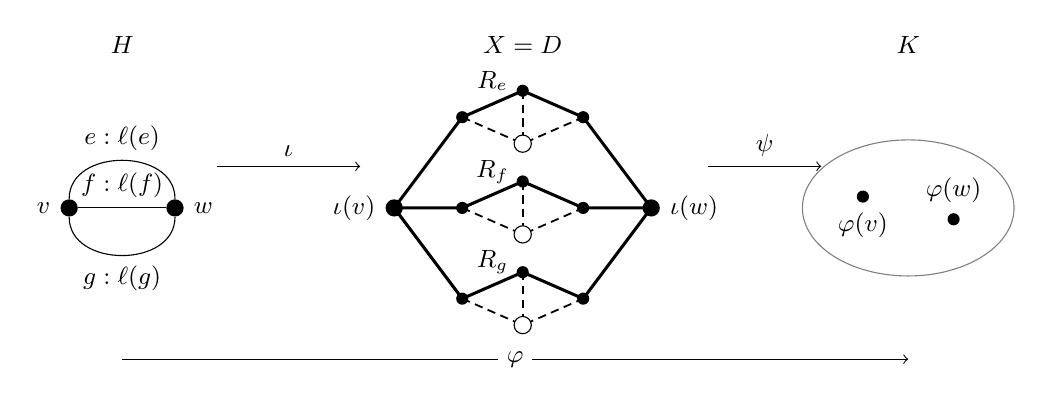
\begin{tikzpicture}[
  x=.96cm,y=.96cm,
  every node/.style={font=\small},
  vertex/.style={circle,fill=black,inner sep=1.55pt},
  branch/.style={circle,fill=black,inner sep=2.2pt},
  outside/.style={circle,draw=black,fill=white,inner sep=2.2pt},
  route/.style={line width=1.1pt},
  perron/.style={densely dashed,line width=.65pt},
]
\node at (0,2.15) {$H$};
\node at (5.3,2.15) {$X=D$};
\node at (10.4,2.15) {$K$};
\node[branch,label=left:$v$] (hu) at (-.7,0) {};
\node[branch,label=right:$w$] (hv) at (.7,0) {};
\draw (hu) .. controls (-.7,.8) and (.7,.8) .. (hv)
  node[midway,above] {$e:\ell(e)$};
\draw (hu)--(hv) node[midway,above] {$f:\ell(f)$};
\draw (hu) .. controls (-.7,-.8) and (.7,-.8) .. (hv)
  node[midway,below] {$g:\ell(g)$};

\coordinate (xu) at (3.6,0);
\coordinate (xv) at (7,0);
\foreach \height/\j in {1.2/e,0/f,-1.2/g} {
  \coordinate (a\j) at (4.5,\height);
  \coordinate (b\j) at (6.1,\height);
  \coordinate (c\j) at (5.3,\height+.35);
  \coordinate (d\j) at (5.3,\height-.35);
  \draw[perron] (a\j)--(d\j)--(b\j);
  \draw[perron] (c\j)--(d\j);
  \draw[route] (xu)--(a\j)--(c\j)--(b\j)--(xv);
  \foreach \p in {a,b,c} {\node[vertex] at (\p\j) {};}
  \node[outside] at (d\j) {};
  \node at (4.9,\height+.48) {$R_\j$};
}
\node[branch,label=left:$\iota(v)$] at (xu) {};
\node[branch,label=right:$\iota(w)$] at (xv) {};

\draw[black!50] (10.4,0) ellipse (1.4 and .9);
\node[vertex,label=below:$\varphi(v)$] at (9.8,.15) {};
\node[vertex,label=above:$\varphi(w)$] at (11,-.15) {};
\draw[->] (1.25,.55)--(3.15,.55) node[midway,above] {$\iota$};
\draw[->] (7.75,.55)--(9.25,.55) node[midway,above] {$\psi$};
\draw[->] (0,-2)--(10.4,-2)
  node[midway,fill=white,inner sep=3pt] {$\varphi$};
\end{tikzpicture}
\caption{The objects in \cref{lem:perron-transfer}, using $D$ from
\cref{fig:diamond-objects}.
Edges of $R_e$ have label $\ell(e)$; each solid path has three internal vertices.
Dashed edges have label $\rho_K$; hollow vertices lie outside all $R_e$.
The target $K$ is schematic, with two vertex images marked.
The coefficient $c_K(X,\ell_X)$ sums over all maps $\psi:V(X)\to V(K)$;
the right side of \cref{eq:perron-transfer} sums over all
$\varphi:V(H)\to V(K)$.
For a fixed $\psi$, we have $\varphi=\psi\circ\iota$.}
\label{fig:perron-objects}
\end{figure}

\begin{proof}
The vertices of $X$ consist of $\iota(V(H))$, the internal vertices of
the paths $R_e$, and the vertices outside all $R_e$.
Since $H$ and $X$ are cubic, the paths occupy all three edge incidences
at every vertex of $\iota(V(H))$. At an internal vertex of $R_e$, two incidences
belong to $R_e$; the third belongs to no chosen path, since their
interiors are disjoint. Every edge incident with a vertex outside all
$R_e$ lies outside the chosen subdivision.

In the sum defining $c_K(X,\ell_X)$, let $\psi:V(X)\to V(K)$ denote
the vertex map and put $\varphi=\psi\circ\iota$.
For each edge $vw$ outside all $R_e$, factor its projector entry as
$P_{\rho_K,K}(\psi(v),\psi(w))=u_K(\psi(v))u_K(\psi(w))$.
Regrouping these factors by their endpoints gives no $u_K$ factor
at vertices of $\iota(V(H))$, one at each internal path vertex, and three at each
vertex outside all $R_e$.
On the paths $R_e$, retain the projector factors $P_{\ell(e),K}$,
including when $\ell(e)=\rho_K$.
Summing over the image of each vertex outside all $R_e$ gives
$\sum_{x\in V(K)}u_K(x)^3=\tau_K$.
There are $|V(X)|-|V(H)|-\sum_eq_e$ such vertices.

For each edge $e=vw$, let $\lambda=\ell(e)$.
Summing over the image of one internal path vertex between fixed
neighbour images $x,y\in V(K)$ gives
\begin{equation}\label{eq:perron-path-factor}
 \sum_{z\in V(K)}P_{\lambda,K}(x,z)u_K(z)P_{\lambda,K}(z,y)
 =M_{\lambda,K}(x,y).
\end{equation}
Let $x_1,\ldots,x_{q_e}$ be the images of the internal vertices of $R_e$,
and put $x_0=\varphi(v)$ and $x_{q_e+1}=\varphi(w)$.
Since $P_{\lambda,K}^2=P_{\lambda,K}$ and $q_e\geq1$, summing over
these images gives
\begin{equation}\label{eq:path-image-sum}
 \sum_{x_1,\ldots,x_{q_e}\in V(K)}
 \left(\prod_{j=0}^{q_e}P_{\lambda,K}(x_j,x_{j+1})\right)
 \left(\prod_{j=1}^{q_e}u_K(x_j)\right)
 =M_{\lambda,K}^{q_e}(\varphi(v),\varphi(w)).
\end{equation}
For a loop $e$, we have $\varphi(v)=\varphi(w)$, so the same calculation gives a diagonal
entry of $M_{\lambda,K}^{q_e}$.
Summing over $\varphi$ now gives
\begin{equation}\label{eq:component-path-sum}
 c_K(X,\ell_X)
 =\tau_K^{|V(X)|-|V(H)|-\sum_eq_e}
   \sum_{\varphi:V(H)\to V(K)}
   \prod_{e=vw\in E(H)}M_{\ell(e),K}^{q_e}(\varphi(v),\varphi(w)).
\end{equation}
Substituting
$M_{\ell(e),K}^{q_e}=\tau_K^{q_e}(M_{\ell(e),K}/\tau_K)^{q_e}$
in \cref{eq:component-path-sum} proves \cref{eq:perron-transfer}.
The total exponent of $\tau_K$ is $|V(X)|-|V(H)|$, independent of the path lengths.
\end{proof}

\begin{lemma}\label{lem:positive-interpolation}
 Let $M_1,\ldots,M_p$ be positive semidefinite operators on finite-dimensional
 Euclidean spaces, and let $P_i$ be the orthogonal projector onto $\im M_i$.
 Suppose their spectra together contain at most $s$ distinct positive values,
 and let $Q$ be a set of at least $s$ distinct positive integers.
 Then there are coefficients $(a_q)_{q\in Q}$, only finitely many nonzero,
 with $\sum_{q\in Q}a_qM_i^q=P_i$ for every $i$.
\end{lemma}
\begin{proof}
 Let $\mu_1,\ldots,\mu_{s'}$ be the distinct positive
 values in the spectra of $M_1,\ldots,M_p$.
 Since $s'\leq s$, we can choose distinct elements $q_1,\ldots,q_{s'}$ of $Q$.
 The generalised Vandermonde matrix $(\mu_h^{q_j})_{h,j=1}^{s'}$ is
 invertible~\cite[p.~76]{GantmacherKrein2002}.
 Hence there are coefficients $a_{q_1},\ldots,a_{q_{s'}}$ with
 $\sum_ja_{q_j}\mu_h^{q_j}=1$ for every $h$; the remaining $a_q$ are zero.
 The operator $\sum_{q\in Q}a_qM_i^q$ is the identity on each positive
 eigenspace and is zero on $\ker M_i$, since every $q$ is positive.
 It therefore equals $P_i$.
\end{proof}

The next lemma combines two interpolations: one replaces operator powers
by image projectors, and the other removes scalar weights.
\begin{lemma}\label{lem:two-stage-interpolation}
 Let $\mathcal I,\mathcal J$ be finite sets. For each $i\in\mathcal I$ and $j\in\mathcal J$, let
 $M_{i,j}$ be a positive semidefinite operator on a finite-dimensional
 Euclidean space $V_{i,j}$, and let $P_{i,j}$ be the orthogonal projector
 onto $\im M_{i,j}$. Let $\Phi_i$ be a multilinear form on
 $\prod_{j\in\mathcal J}\operatorname{End}(V_{i,j})$, and let
 $\tau_i>0$ and $\varepsilon_i\in\R$.
 Let $(d_N)$ be an unbounded sequence of nonnegative integers.
 Suppose that, for every sufficiently large $N$, there are finite
 sets $Q_{N,j}\subseteq\Z_{\geq1}$ with
 $|Q_{N,j}|\geq\sum_{i\in\mathcal I}\dim V_{i,j}$,
 such that
 \begin{equation}\label{eq:two-stage-samples}
  \sum_{i\in\mathcal I}\varepsilon_i\tau_i^{d_N}
     \Phi_i((M_{i,j}^{q_j})_{j\in\mathcal J})=0
  \quad\text{for every }\mathbf q\in\prod_{j\in\mathcal J}Q_{N,j}.
 \end{equation}
 Then $\sum_{i\in\mathcal I}\varepsilon_i\Phi_i((P_{i,j})_{j\in\mathcal J})=0$.
\end{lemma}
\begin{proof}
 For each $j\in\mathcal J$, the spectra of the operators $(M_{i,j})_{i\in\mathcal I}$
 together contain at most $\sum_{i\in\mathcal I}\dim V_{i,j}$ distinct positive
 values. Thus, for each sufficiently large $N$ and each $j$,
 \cref{lem:positive-interpolation} gives coefficients $a_{N,j,q}$ with
 $\sum_{q\in Q_{N,j}}a_{N,j,q}M_{i,j}^q=P_{i,j}$ for every $i$.
 By multilinearity,
 \begin{equation}\label{eq:two-stage-operators}
  \sum_i\varepsilon_i\tau_i^{d_N}\Phi_i((P_{i,j})_j)
  =\sum_{\mathbf q\in\prod_jQ_{N,j}}
      \left(\prod_ja_{N,j,q_j}\right)
      \sum_i\varepsilon_i\tau_i^{d_N}\Phi_i((M_{i,j}^{q_j})_j)=0.
 \end{equation}
 Since $d_N$ is unbounded, we can choose $|\mathcal I|$ sufficiently large indices $N_h$
 with distinct positive values of $d_{N_h}$.
 Applying \cref{lem:positive-interpolation} to the operators
 $t\mapsto\tau_i t$ on $\R$ with these exponents gives coefficients $b_h$
 with $\sum_hb_h\tau_i^{d_{N_h}}=1$ for every $i$.
 Summing \cref{eq:two-stage-operators} at these indices with
 coefficients $b_h$ proves the lemma.
\end{proof}

\begin{lemma}\label{lem:cubic-coefficient-transfer}
 Let $(H_N)_{N\geq1}$ be a sequence of connected cubic graphs such that
 $H_N$ contains $K_{3N}$ as a minor for every $N\geq1$.
 Let $G,G'$ be finite simple graphs. Suppose
 $c_G(H_N,\ell)=c_{G'}(H_N,\ell)$ for every $N\geq1$ and every
 labelling $\ell:E(H_N)\to\R^\times$.
 Then $c_G(H,\ell)=c_{G'}(H,\ell)$ for every connected cubic
 multigraph $H$ and every labelling $\ell:E(H)\to\R^\times$.
\end{lemma}
\begin{proof}
For every graph $G$, connected multigraph $H$ with an edge, and nonzero
edge labelling $\ell$, we have
\begin{equation}\label{eq:component-contributions}
 c_G(H,\ell)=\sum_K c_K(H,\ell),
\end{equation}
where $K$ ranges over the connected components of $G$.
Indeed, the spectral projectors of $A_G$ are block diagonal over these
components, so a map $V(H)\to V(G)$ contributes zero unless its image
lies in one component.
For a component $K$, a label $\lambda>\rho_K$ on any edge gives
$c_K(H,\ell)=0$, because $P_{\lambda,K}=0$.

Fix an integer $n\geq0$. We prove the lemma for all pairs $G,G'$ with
$|V(G)|+|V(G')|\leq2n$.
The combined vertex bound allows the two graphs to have different
numbers of vertices after components are deleted.
We argue by induction on the total number of components containing an edge.
If both graphs are edgeless, including when either has no vertices,
every labelled coefficient of a connected cubic multigraph is zero.
Otherwise $n\geq1$. Let $r>0$ be the largest spectral radius among all
components of both graphs, and let $\mathcal K,\mathcal K'$ consist of
the components of $G,G'$, respectively, with spectral radius $r$.
Since $r$ is attained, $\mathcal K\sqcup\mathcal K'\ne\varnothing$.
Fix a connected cubic multigraph $H$ and a nonzero edge labelling $\ell$.
We prove that
\begin{equation}\label{eq:layer-contractions}
 \sum_{K\in\mathcal K}c_K(H,\ell)
 =\sum_{K\in\mathcal K'}c_K(H,\ell).
\end{equation}
Apply \cref{lem:independent-path-lengths} with $m=2n$ to obtain $D$.
For every sufficiently large $N$, \cref{lem:subdivision-containment}
places a subdivision of $D$ in $H_N$.
Hence \cref{lem:independent-path-lengths} supplies an injection
$\iota:V(H)\hookrightarrow V(H_N)$ and sets
$Q_e\subseteq\Z_{\geq1}$ with $|Q_e|\geq2n+1$.
For each $\mathbf q\in\prod_eQ_e$, choose the paths $R_e$ given by that
lemma. Let $\ell_N(\mathbf q)$ assign $\ell(e)$ to the edges of $R_e$
and $r$ to every edge outside the paths.
This is the labelling $\ell_X$ in \cref{lem:perron-transfer} with
$X=H_N$ and $\rho_K=r$.
At least one edge receives $r$, so only components in $\mathcal K$
contribute to $c_G(H_N,\ell_N(\mathbf q))$.
Put $n_N=|V(H_N)|$ and $n_H=|V(H)|$.
Since $\rho_K=r$ for every $K\in\mathcal K$, applying
\cref{lem:perron-transfer} to each such $K$ and using
\cref{eq:component-contributions} gives
\begin{equation}\label{eq:operator-transfer}
 c_G(H_N,\ell_N(\mathbf q))=\sum_{K\in\mathcal K}\tau_K^{n_N-n_H}
   \sum_{\varphi:V(H)\to V(K)}
   \prod_{e=vw\in E(H)}
       \left(\frac{M_{\ell(e),K}}{\tau_K}\right)^{q_e}(\varphi(v),\varphi(w)).
\end{equation}
The same labelling satisfies \cref{eq:operator-transfer} for $G'$ and
$\mathcal K'$ because every $K\in\mathcal K'$ also has $\rho_K=r$.
We suppress the dependence of the sets $Q_e$ on $N$.
Interpolation over $q_e$ in \cref{eq:operator-transfer} will replace
$(M_{\ell(e),K}/\tau_K)^{q_e}$ by $P_{\ell(e),K}$.
Interpolation over $N$ will then replace $\tau_K^{n_N-n_H}$ by $1$.

We apply \cref{lem:two-stage-interpolation} with component index set
$\mathcal I=\mathcal K\sqcup\mathcal K'$ and edge index set $\mathcal J=E(H)$.
The signs are $+1$ on $\mathcal K$ and $-1$ on $\mathcal K'$.
For each component $K$ and edge $e$, the operator is
$M_{\ell(e),K}/\tau_K$ on $\R^{V(K)}$.
It is positive semidefinite with image projector $P_{\ell(e),K}$.
For each component $K$, let
\begin{equation}\label{eq:component-multilinear-form}
 \Phi_K((T_e)_{e\in E(H)})
 =\sum_{\varphi:V(H)\to V(K)}
   \prod_{e=vw\in E(H)}T_e(\varphi(v),\varphi(w)),
\end{equation}
where each $T_e$ is a matrix indexed by $V(K)$.
This form is multilinear, and $\Phi_K((P_{\ell(e),K})_e)=c_K(H,\ell)$.
The spaces $\R^{V(K)}$ have total dimension
$\sum_{K\in\mathcal K\sqcup\mathcal K'}|V(K)|\leq2n$.
Every $Q_e$ has at least $2n+1$ elements, so the dimension bound
in \cref{lem:two-stage-interpolation} holds.
The assumed equality of the two instances of \cref{eq:operator-transfer}
is exactly \cref{eq:two-stage-samples} with $d_N=n_N-n_H$.
Since $H_N$ contains a $K_{3N}$ minor, $n_N\geq3N$.
Thus $d_N$ is nonnegative for all sufficiently large $N$ and is unbounded.
Hence \cref{lem:two-stage-interpolation} proves \cref{eq:layer-contractions}.

Let $G^-$ and $G'^-$ be obtained by deleting the components in
$\mathcal K$ and $\mathcal K'$, respectively.
Let $N_\ast\geq1$ and let $\eta$ be a nonzero labelling of $H_{N_\ast}$.
Since $H_{N_\ast}$ is connected and cubic, \cref{eq:layer-contractions} holds
with $H=H_{N_\ast}$ and $\ell=\eta$, so by \cref{eq:component-contributions}
and the assumed equality on $H_{N_\ast}$,
\begin{equation}\label{eq:residual-contractions}
 \begin{aligned}
 c_{G^-}(H_{N_\ast},\eta)
 &=c_G(H_{N_\ast},\eta)-\sum_{K\in\mathcal K}c_K(H_{N_\ast},\eta)\\
 &=c_{G'}(H_{N_\ast},\eta)-\sum_{K\in\mathcal K'}c_K(H_{N_\ast},\eta)
 =c_{G'^-}(H_{N_\ast},\eta).
 \end{aligned}
\end{equation}
We have $|V(G^-)|+|V(G'^-)|\leq2n$.
Since $\mathcal K\sqcup\mathcal K'\ne\varnothing$ and $r>0$, deleting
these components strictly decreases the total number containing an edge.
The induction hypothesis therefore gives
$c_{G^-}(H,\ell)=c_{G'^-}(H,\ell)$ for every connected cubic $H$ and
nonzero labelling $\ell$.
Adding the equal sums in \cref{eq:layer-contractions} and using
\cref{eq:component-contributions} gives $c_G(H,\ell)=c_{G'}(H,\ell)$,
proving the lemma.
\end{proof}

\begin{proof}[Proof of \cref{prop:closure}]
By the initial reduction, it suffices to prove the equivalence for $\calF'$.
Suppose $G\equiv_{\calF'}G'$. Since $K_1\in\calF'$, we have
$|V(G)|=|V(G')|$.
Their counts agree on every subdivision $H_N^{\mathbf m}$.
By \cref{lem:subdivision-coefficients},
$c_G(H_N,\ell)=c_{G'}(H_N,\ell)$ for every $N$ and every nonzero labelling $\ell$.
\Cref{lem:cubic-coefficient-transfer} therefore gives equality of the labelled
coefficients on every connected cubic multigraph. By \cref{lem:characterisation}(c),
$G\equiv_{\mathcal D_3}G'$.
The reverse implication follows from $\calF'\subseteq\mathcal D_3$,
and completeness on simple spectrum follows from \cref{thm:main}.
\end{proof}
